\documentclass[
    fontsize=12pt,          % default font size 12pt
    paper=a4,               % DIN A4 page format
    numbers=noenddot,       % remove dots behind chapter numbers (e.g. 1.5 not 1.5.)
    listof=totoc,           % add list of figures, tables, etc. to ToC
    listof=entryprefix,     % add entry name to figures, tables, etc.
    listof=nochaptergap,    % no chapter gap for figures, tables, etc.
    bibliography=totoc,     % add bibliography to ToC but without a chapter number
    parskip=half,           % half line spacing between paragraphs
    openany                 % chapters can start on any page
]{scrbook}

\include{../../for_latex/preamble}

\begin{document}

    \begin{titlepage}
    	\pagestyle{empty}
    	
    	% HFU Logo
    	\begin{flushright}
    		\begin{figure}[ht]
    			\flushright
    			
\includegraphics[height=2cm]{../../for_latex/hfu}
    		\end{figure}
    	\end{flushright}
    	
    	\begin{center}
    		\vspace{3cm}
    		
    		{\fontsize{22}{22} \selectfont \textbf{Blatt 5}}\\[5mm]
    		{\fontsize{18}{18} \selectfont Kryptologie}
    		
    		\vspace{12cm}
    		
    		{\fontsize{14}{14} \selectfont Luis Staudt}
    	\end{center}
    \end{titlepage}

% ############################################################################
% CONTENT STARTS HERE
% ############################################################################


\chapter*{Performance-Vergleich: DLP $-$ ECDLP}


\section*{Aufgabenstellung}

Verglichen werden soll der Aufwand der \textbf{Schlüsselpaar-Erzeugung} $(a, A)$ für zwei
auf dem diskreten Logarithmus beruhende Verfahren bei \emph{gleichem Sicherheitsniveau}~$k$
gemäß BSI TR-02102-1:

\begin{itemize}
    \item \textbf{Klassisches DLP} in $\mathrm{GF}(p)$: modulare Exponentiation $A := G^a \bmod p$,
          wobei die Primzahl $p$ eine Bitlänge von $N$ besitzt.
    \item \textbf{ECDLP}: skalare Multiplikation $A := [a]\,G$ auf einer elliptischen Kurve
          über $\mathrm{GF}(p)$ mit Körper-Bitlänge $n$.
\end{itemize}

Für jedes Sicherheitsniveau~$k$ wird ein zufälliger Parametersatz mit Generator~$G$ erzeugt,
für viele zufällige~$a$ der Punkt~$A$ berechnet und die Laufzeit gemessen. Die Ergebnisse werden
als Boxplots und Vergleichsdiagramme dargestellt und beurteilt.

\begin{table}[H]
    \centering
    \small
    \begin{tabular}{l r r r r r r r r r r r}
        \toprule
        \textbf{Sicherheit} $k$        & 16 & 32 & 56 & 60 & 64 & 70 & 100 & 120 & 128 & 192 & 256 \\
        \midrule
        \textbf{ECDLP} $n$ (Bit)       & 32 & 64 & 112 & 120 & 128 & 140 & 200 & 240 & 256 & 384 & 512 \\
        \textbf{GF$(p)$} $N$ (Bit)     & 64 & 256 & 512 & 700 & 816 & 1000 & 1900 & 2800 & 3200 & 7900 & 15500 \\
        \bottomrule
    \end{tabular}
    \caption{Äquivalente Schlüssellängen gemäß BSI TR-02102-1.}
\end{table}


\section*{Vorgehensweise}

\begin{enumerate}
    \item \textbf{Parametersatz (a):} Pro Bitlänge wird einmalig ein zufälliger Parametersatz erzeugt.
          \begin{itemize}
              \item GF$(p)$: zufällige Primzahl $p$ ($N$ Bit) und ein zufälliger Generator $G \in [2, p-1)$.
              \item EC: zufällige Primzahl $p$ ($n$ Bit) mit $p \equiv 3 \bmod 4$, zufälliger Kurvenparameter $a$
                    und ein zufälliger Punkt $G=(x,y)$; der Parameter $b$ wird so gesetzt, dass $G$ auf der Kurve
                    $y^2 = x^3 + ax + b$ liegt.
          \end{itemize}
    \item \textbf{Berechnung (b):} Für je einen frischen Zufallswert $a$ (Bitlänge $N$ bzw.\ $n$) wird
          $A := G^a \bmod p$ bzw.\ $A := [a]\,G$ berechnet.
    \item \textbf{Messung (c):} Nach einer JIT-Aufwärmphase werden die Laufzeiten oft wiederholt gemessen
          (1000 Wiederholungen, für die sehr großen Körper $N \ge 1900$ aus Zeitgründen reduziert auf
          200 bzw.\ 50). Sehr kurze Operationen werden in einer inneren Schleife gebündelt und gemittelt,
          damit die Messung über der Zeitgeber-Auflösung liegt.
\end{enumerate}

Die Implementierung erfolgt in \textbf{Java}. Die modulare Exponentiation nutzt das Standard-Primitiv
\texttt{java.math.BigInteger.modPow} (Montgomery-Reduktion). Die EC-Punktarithmetik wird
\textbf{nicht selbst implementiert}, sondern der erprobten und optimierten Bibliothek
\textbf{Bouncy Castle} (\texttt{org.bouncyc\-astle.math.ec}) überlassen; selbstgeschriebene
Gruppengesetze sind in einem Benchmark fehleranfällig (Sonderfälle, Formeln) und würden das Ergebnis
verfälschen. Lediglich der \emph{Parametersatz} (Primkörper, Kurvenkoeffizient, Generatorpunkt) wird
selbst zufällig erzeugt, da die BSI-Bitlängen überwiegend keinen standardisierten Kurven entsprechen.
Die statistische Auswertung und die Diagramme werden mit \textbf{Python} (\texttt{matplotlib}) erzeugt.

\begin{lstlisting}[language=Java, caption={Parametersatz und skalare Multiplikation via Bouncy Castle}]
// b so waehlen, dass G = (gx, gy) auf y^2 = x^3 + a*x + b liegt:
BigInteger b = gy.multiply(gy)
    .subtract(gx.modPow(THREE, p)).subtract(a.multiply(gx)).mod(p);
ECCurve curve = new ECCurve.Fp(p, a, b, null, null);   // Ordnung/Kofaktor irrelevant
ECPoint   G     = curve.createPoint(gx, gy);

ECPoint A = G.multiply(scalar).normalize();            // A := [a]G
\end{lstlisting}


\section*{Ergebnisse}

Tabelle~\ref{tab:median} fasst die Median-Laufzeiten pro Operation zusammen. Der Faktor gibt an,
um wie viel die EC-Variante schneller (Faktor $>1$) bzw.\ langsamer (Faktor $<1$) als die
modulare Exponentiation bei gleichem Sicherheitsniveau ist.

\begin{table}[H]
    \centering
    \begin{tabular}{r r r r r r}
        \toprule
        $k$ & $n$ (Bit) & $N$ (Bit) & \textbf{EC} $[a]G$ ($\mu$s) & \textbf{GF$(p)$} $G^a$ ($\mu$s) & \textbf{Faktor} \\
        \midrule
         16 &  32 &    64 &      12{,}8 &        1{,}0 & 0{,}1$\times$ \\
         32 &  64 &   256 &      49{,}6 &        8{,}5 & 0{,}2$\times$ \\
         56 & 112 &   512 &     171{,}4 &       39{,}1 & 0{,}2$\times$ \\
         60 & 120 &   700 &     169{,}8 &       86{,}6 & 0{,}5$\times$ \\
         64 & 128 &   816 &     172{,}7 &      133{,}5 & 0{,}8$\times$ \\
         70 & 140 &  1000 &     218{,}8 &      233{,}7 & 1{,}1$\times$ \\
        100 & 200 &  1900 &     464{,}2 &     1\,377{,}7 & \textbf{3{,}0$\times$} \\
        120 & 240 &  2800 &     624{,}2 &     4\,027{,}5 & \textbf{6{,}5$\times$} \\
        128 & 256 &  3200 &     624{,}3 &     5\,879{,}3 & \textbf{9{,}4$\times$} \\
        192 & 384 &  7900 &   1\,475{,}4 &    88\,034{,}1 & \textbf{59{,}7$\times$} \\
        256 & 512 & 15500 &   2\,983{,}1 &   658\,821{,}3 & \textbf{220{,}9$\times$} \\
        \bottomrule
    \end{tabular}
    \caption{Median-Laufzeiten pro Schlüsselpaar-Erzeugung und Geschwindigkeitsfaktor.}
    \label{tab:median}
\end{table}

\begin{figure}[H]
    \centering
    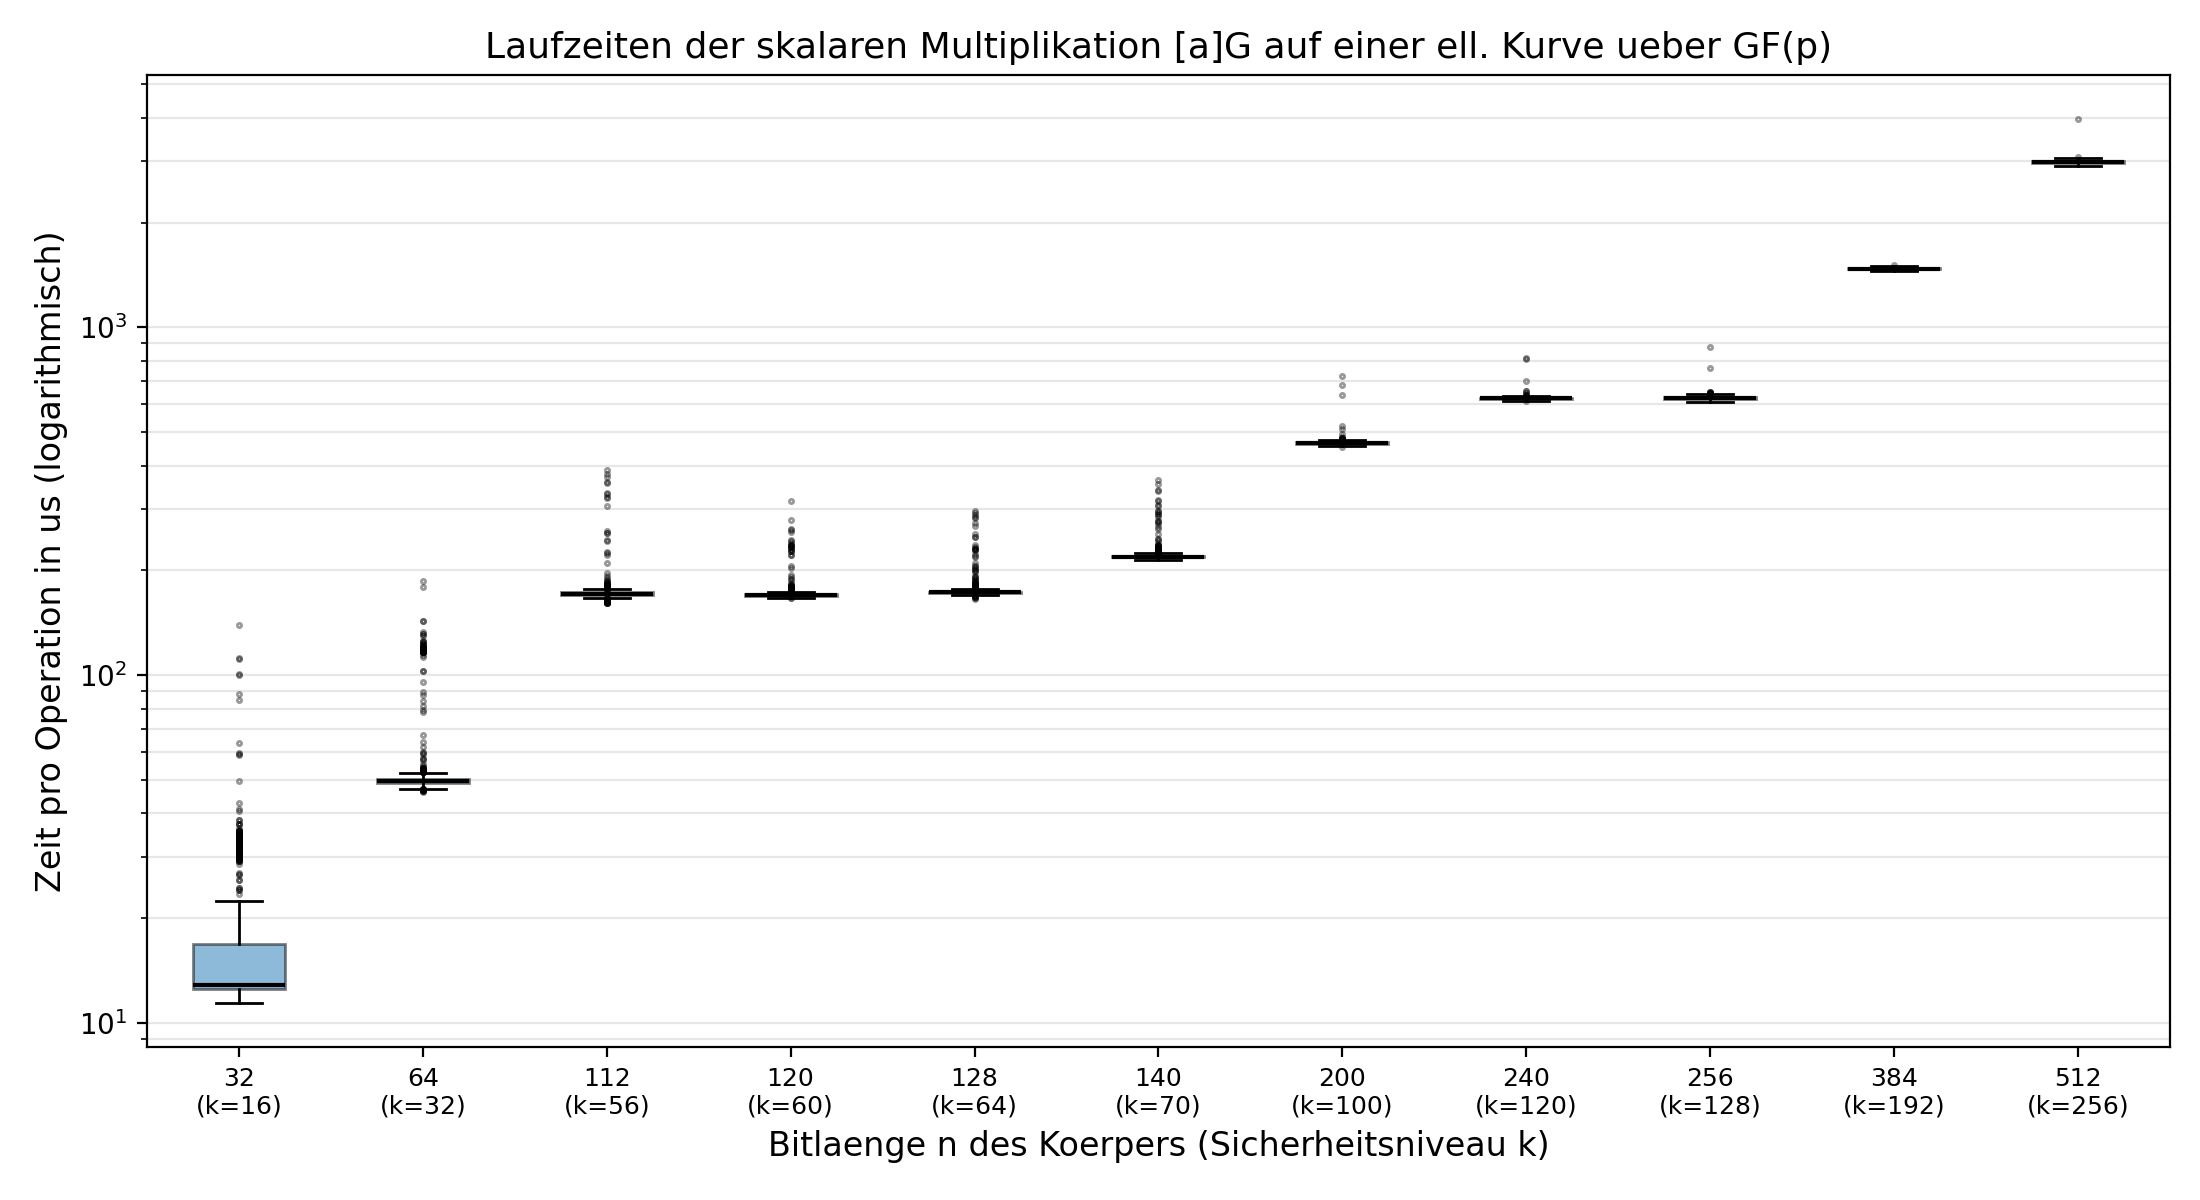
\includegraphics[width=\linewidth]{boxplot_ec.png}
    \caption{Laufzeiten der skalaren Multiplikation $[a]G$ (ECDLP) je Bitlänge $n$.}
\end{figure}

\begin{figure}[H]
    \centering
    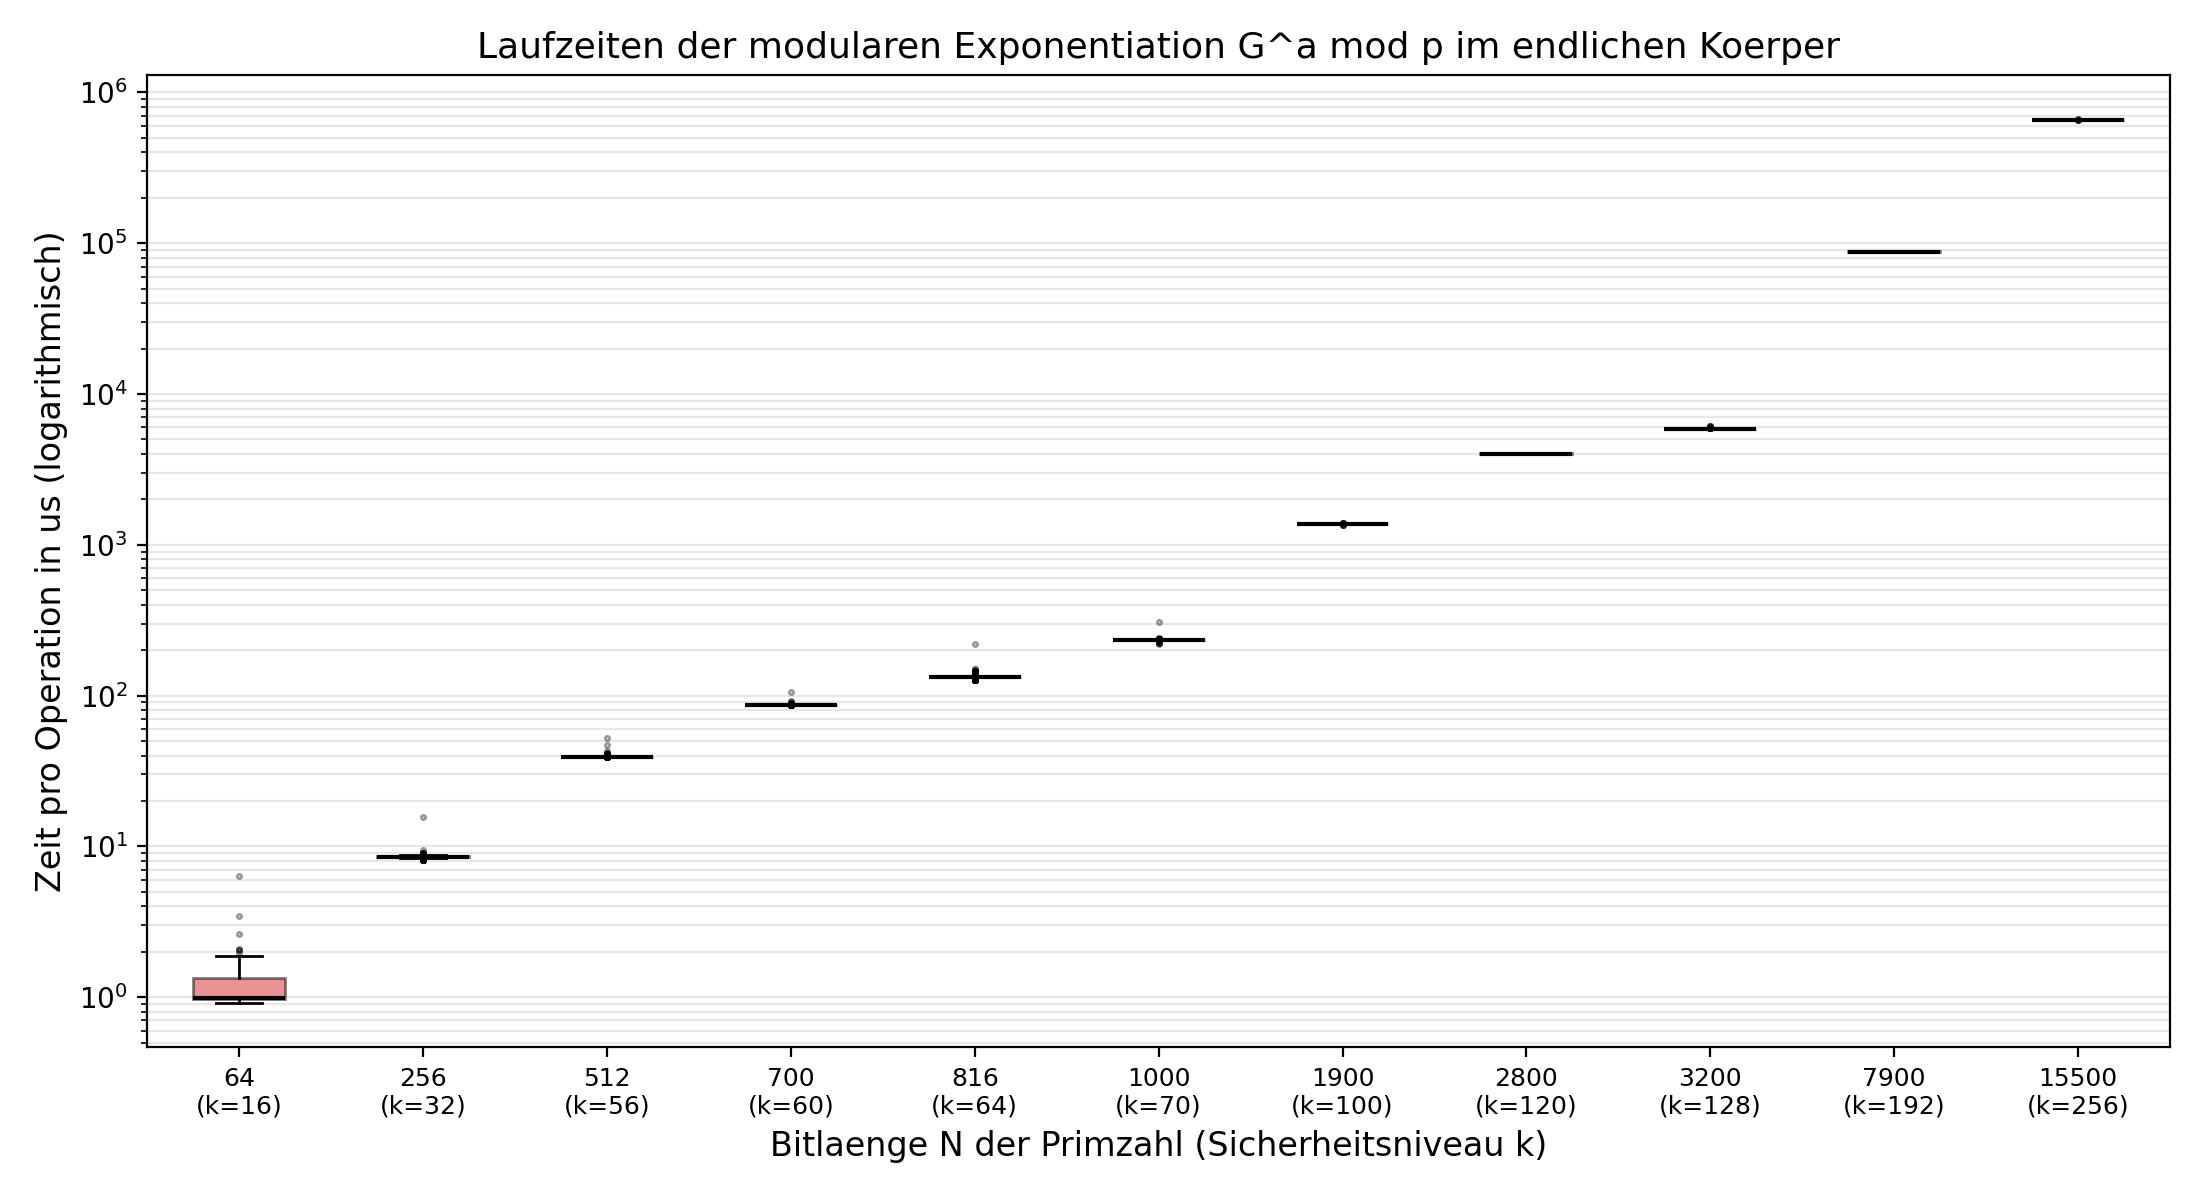
\includegraphics[width=\linewidth]{boxplot_gf.png}
    \caption{Laufzeiten der modularen Exponentiation $G^a \bmod p$ (DLP) je Bitlänge $N$.}
\end{figure}

\begin{figure}[H]
    \centering
    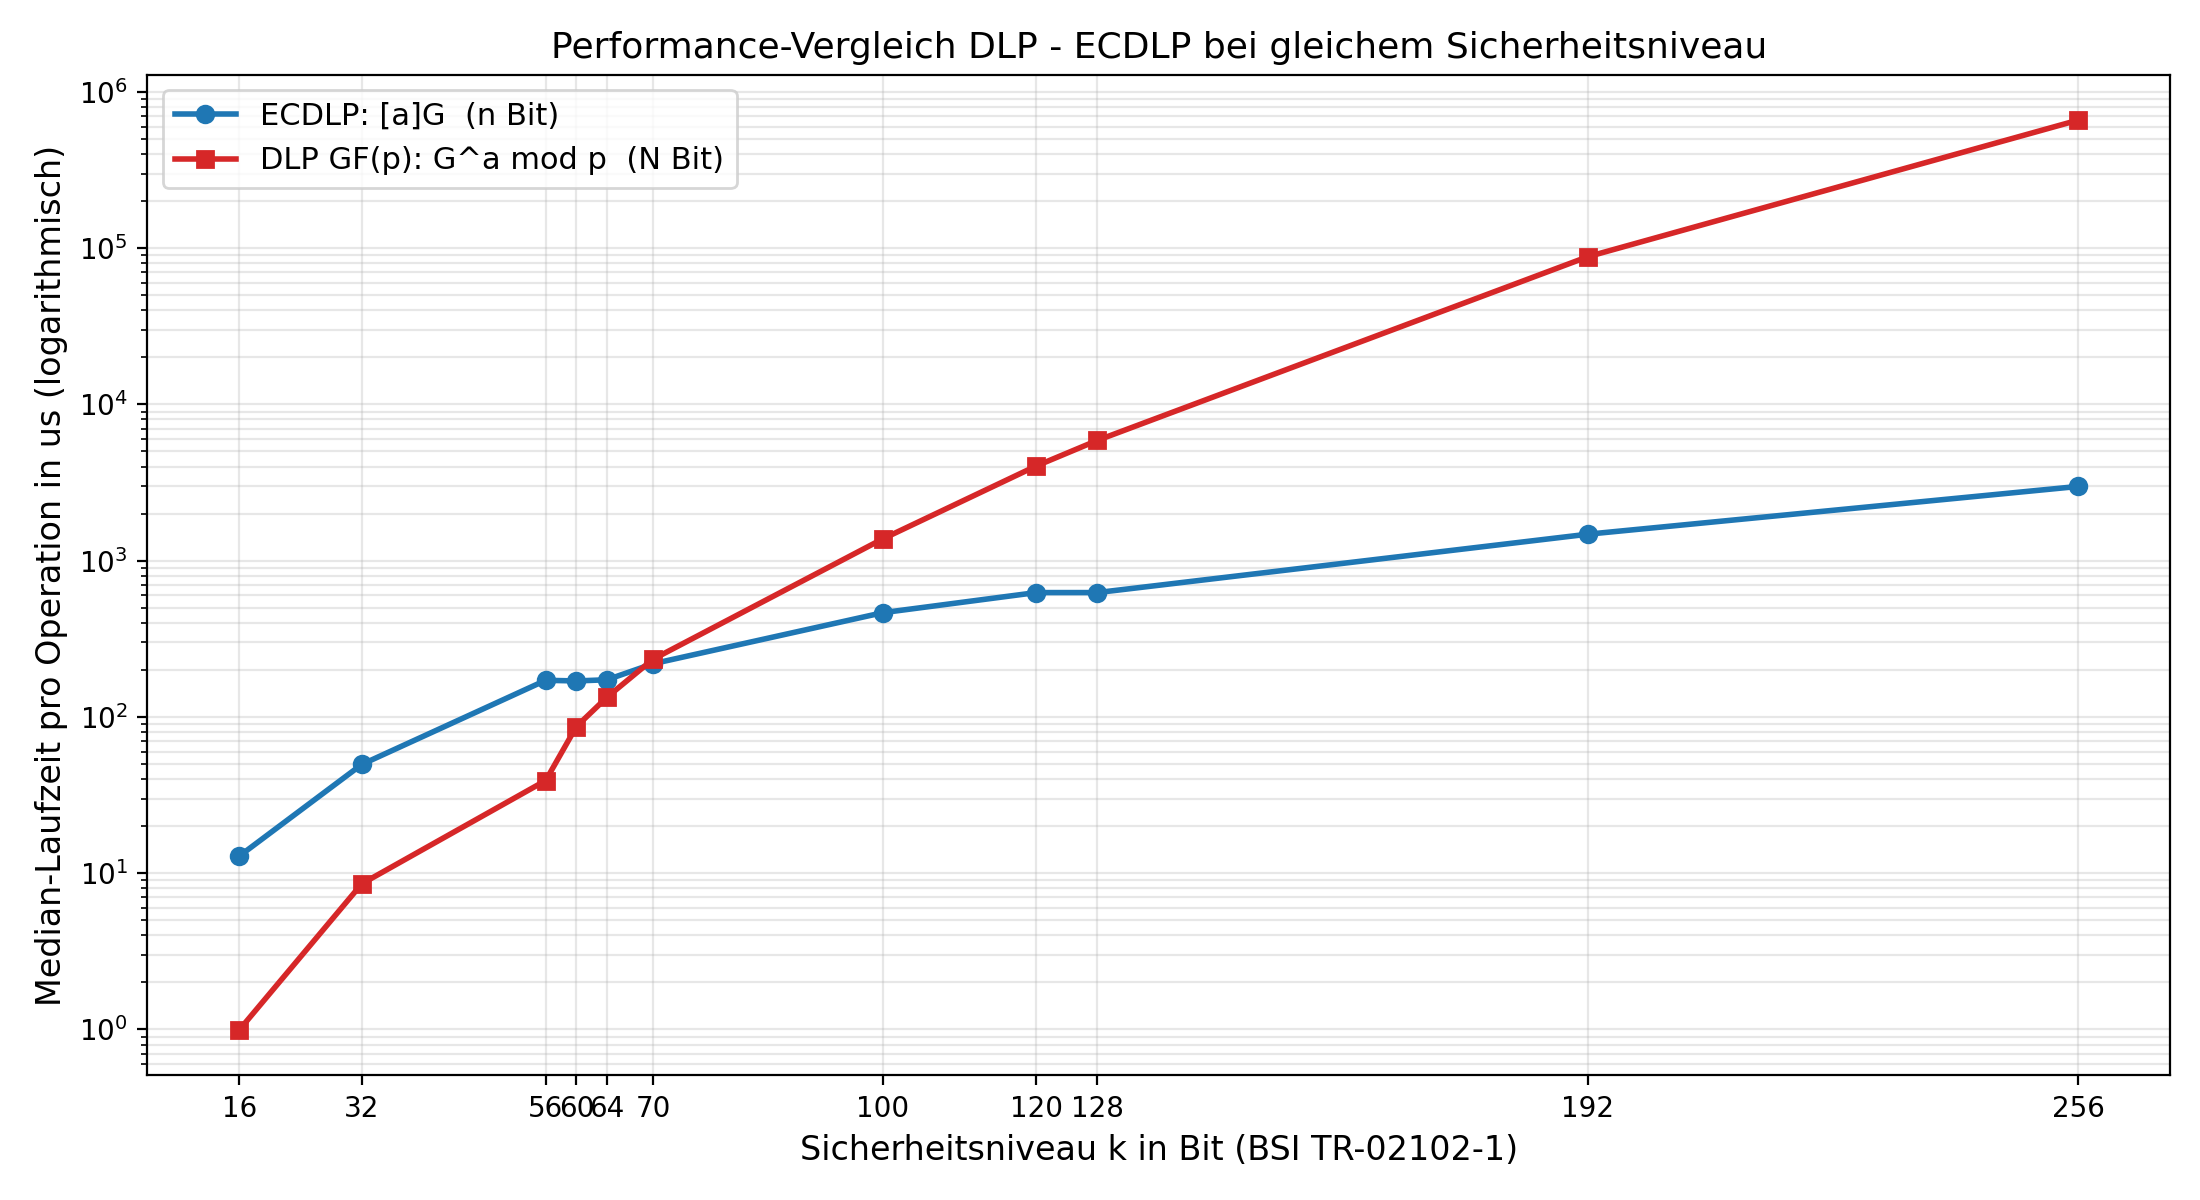
\includegraphics[width=\linewidth]{comparison_median.png}
    \caption{Direkter Vergleich der Median-Laufzeiten über das Sicherheitsniveau~$k$ (log.\ Skala).
             Der Schnittpunkt der beiden Kurven liegt bei $k \approx 70$.}
\end{figure}

\begin{figure}[H]
    \centering
    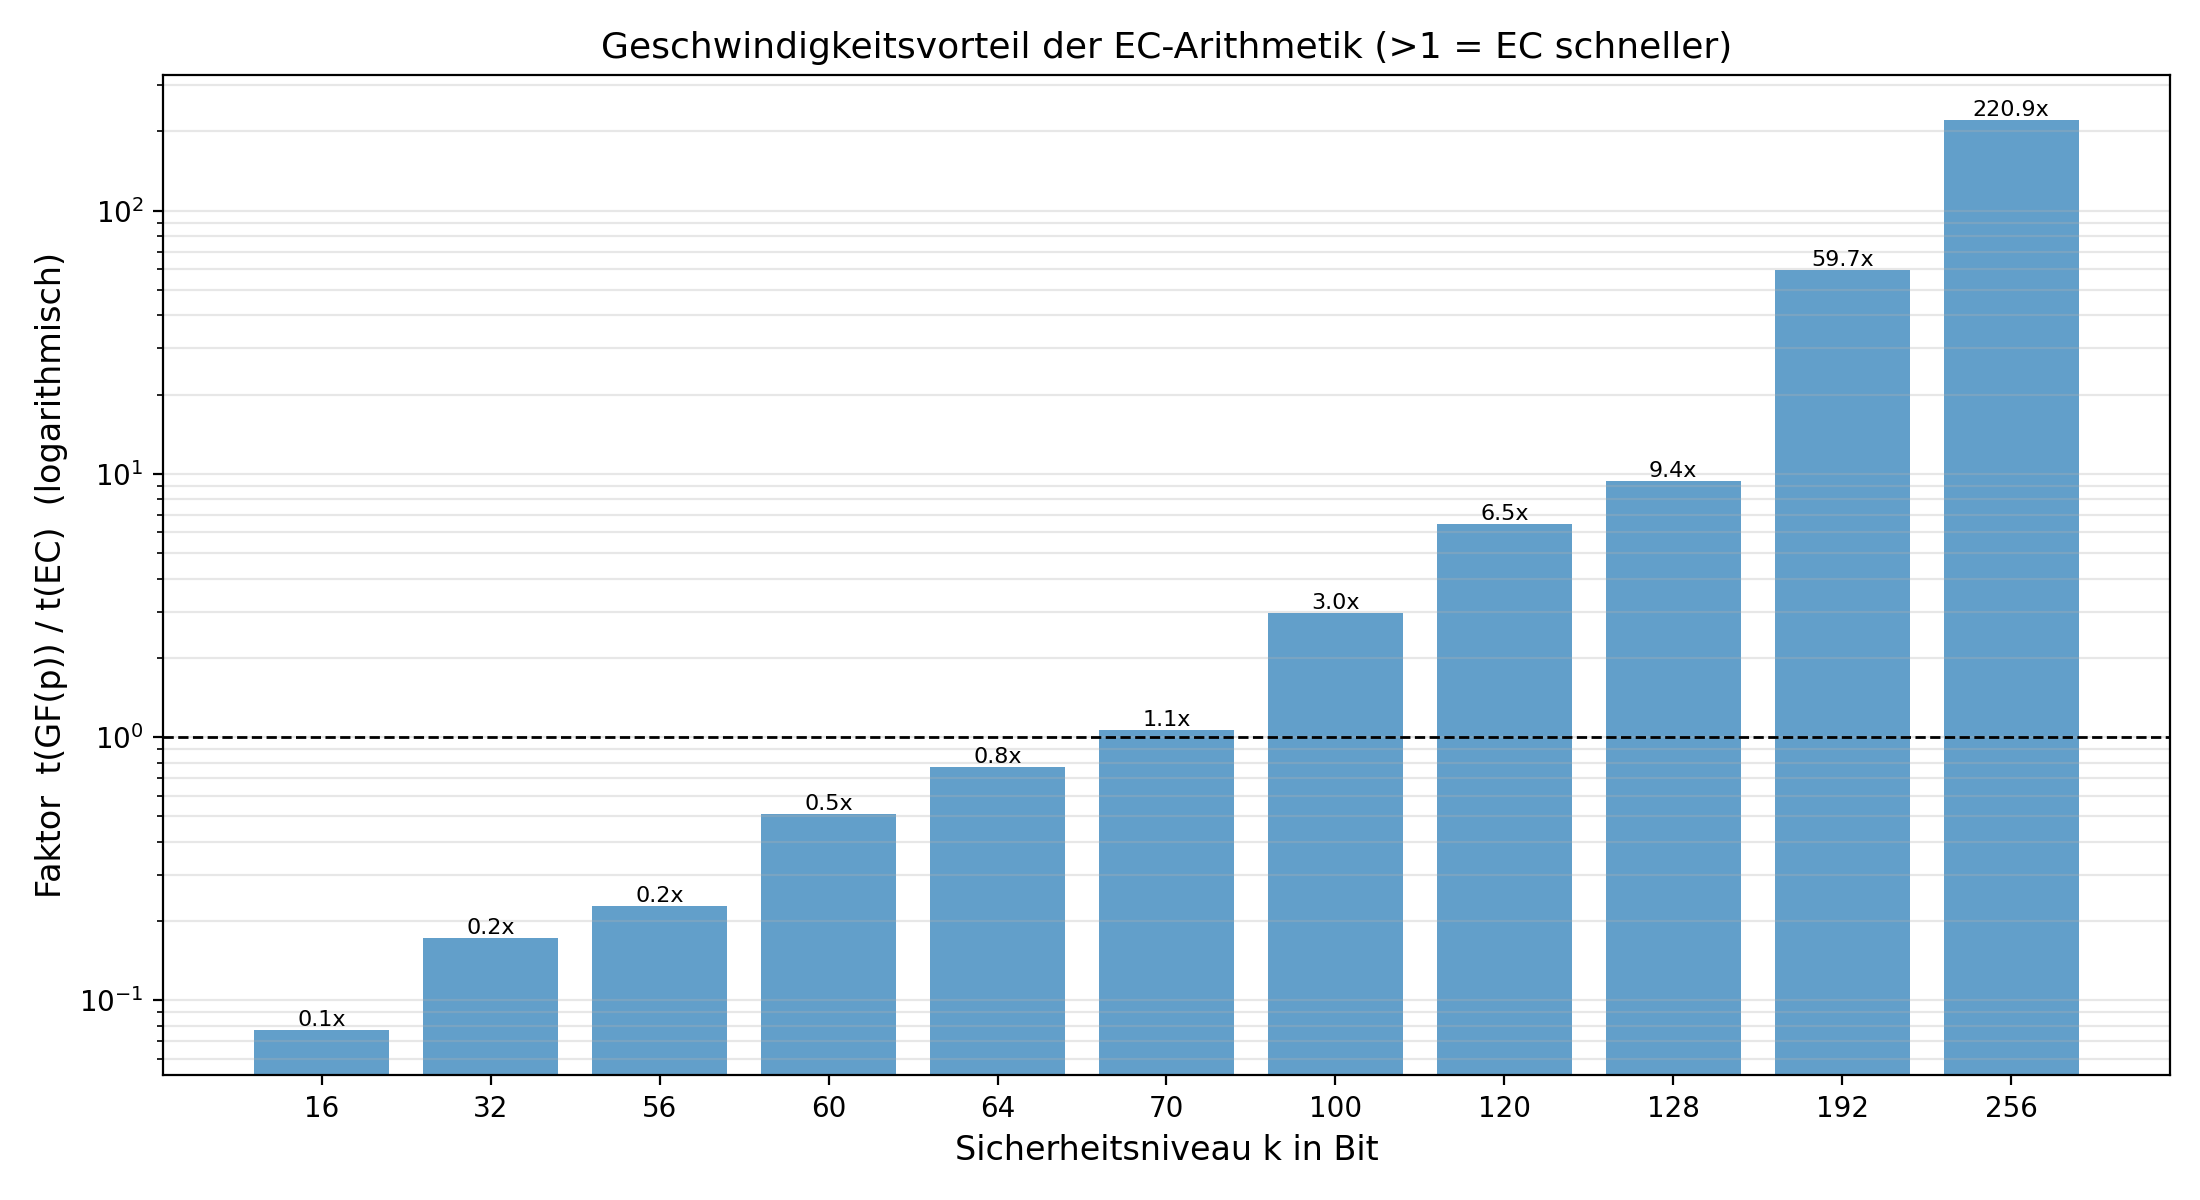
\includegraphics[width=\linewidth]{speedup.png}
    \caption{Geschwindigkeitsvorteil der EC-Arithmetik: Verhältnis $t(\mathrm{GF}(p)) / t(\mathrm{EC})$.}
\end{figure}


\section*{Auswertung}

\subsection*{Komplexität}

Beide Operationen folgen einem \texttt{square-/double-and-add}-Schema mit kubischem Aufwand in der
Bitlänge:
\begin{itemize}
    \item \textbf{Modulare Exponentiation} $G^a \bmod p$: ca.\ $N$ modulare Multiplikationen mit je
          $\mathcal{O}(N^2)$ $\Rightarrow$ $\mathcal{O}(N^3)$.
    \item \textbf{Skalare Multiplikation} $[a]G$: ca.\ $n$ Punktoperationen mit je konstant vielen
          Körpermultiplikationen $\mathcal{O}(n^2)$ $\Rightarrow$ $\mathcal{O}(n^3)$.
\end{itemize}
Da bei gleichem Sicherheitsniveau $N \gg n$ gilt (z.\,B.\ $N=3200$ gegenüber $n=256$ bei $k=128$),
ist der Aufwand der EC-Variante asymptotisch um den Faktor $(N/n)^3$ geringer.

\subsection*{Beobachtetes Verhalten}

\begin{itemize}
    \item \textbf{Kleine Sicherheitsniveaus ($k \le 64$):} Hier ist die modulare Exponentiation sogar
          \emph{schneller}. Die Körper sind klein genug, dass die hochoptimierte \texttt{BigInteger.modPow}
          (Montgomery-Reduktion) gegenüber dem höheren Konstantenaufwand einer Punktoperation (mehrere
          Körpermultiplikationen pro Schritt) im Vorteil ist. Bei $k=16$ ist GF$(p)$ rund $13\times$ schneller.
    \item \textbf{Schnittpunkt:} Bei $k \approx 70$ ($n=140$, $N=1000$) sind beide Verfahren etwa
          gleich schnell (Faktor $1{,}1$).
    \item \textbf{Praxisrelevante Niveaus ($k \ge 100$):} Ab hier dominiert die EC-Arithmetik klar.
          Der Vorsprung wächst von $3{,}0\times$ ($k=100$) über $9{,}4\times$ ($k=128$) bis auf
          $221\times$ ($k=256$). Genau dieses überproportionale Auseinanderlaufen wird durch das
          kubische Wachstum bei stark unterschiedlichen Bitlängen erklärt.
\end{itemize}

\subsection*{Streuung}

Die Boxplots zeigen für beide Verfahren eine sehr geringe Streuung um den Median; die wenigen Ausreißer
nach oben sind auf Garbage-Collection und Scheduling der JVM zurückzuführen. Die Laufzeit hängt
praktisch nur von der Bitlänge ab und ist gegenüber dem konkreten Zufallswert $a$ nahezu konstant.


\section*{Bewertung}

Die Messungen bestätigen die in der Einführung genannten Vorteile der EC-Kryptographie quantitativ:
Bei \emph{gleichem Sicherheitsniveau} benötigt die elliptische Kurve eine drastisch kürzere
Schlüssellänge ($n=512$ statt $N=15500$ Bit bei $k=256$) und ist dadurch bei der
Schlüsselpaar-Erzeugung um \textbf{mehr als zwei Größenordnungen} schneller.

Der Vorteil ist nicht konstant, sondern wächst mit dem Sicherheitsniveau: Während bei niedrigen
Niveaus die ausgereifte Implementierung der modularen Exponentiation noch überwiegt, kehrt sich das
Bild ab praxisrelevanten Niveaus ($k \ge 100$) deutlich um. Hinzu kommen die kürzeren Schlüssel,
die Speicherplatz und Bandbreite sparen -- entscheidende Vorteile auf ressourcenbeschränkten Geräten.
Damit erklärt sich, warum moderne Verfahren (z.\,B.\ ECDH, ECDSA) elliptische Kurven gegenüber
klassischen $\mathrm{GF}(p)$-Verfahren bevorzugen.

\emph{Anmerkung zur Methodik:} Es wurde der ungünstigste Fall einer Exponenten-Bitlänge $=N$ gemessen.
In Schnorr-/DSA-Gruppen mit Untergruppe der Ordnung $\approx 2k$~Bit wäre der Exponent kürzer; der
qualitative Befund (überproportionaler EC-Vorteil bei hohen Niveaus) bliebe jedoch bestehen, da die
Kosten einer einzelnen modularen Multiplikation weiterhin $\mathcal{O}(N^2)$ betragen.

% ############################################################################
% CONTENT ENDS HERE
% ############################################################################

\end{document}
